\subsection{Introduction}
The term \textbf{burst} lacks a formal definition. However, it is generally employed to indicate a recording period during which the spiking frequency is especially high, alternating with periods exhibiting a low spiking frequency (quiescence periods).
\begin{figure}[H]
    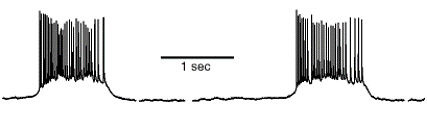
\includegraphics[scale=1]{5_1}
    \centering
\end{figure}
Neural bursting plays a key role in communication between neurons, in particular
burst neurons are crucial in \textbf{motor pattern generation and synchronization}.
A burst doesn't necessarily come from a network of neurons, but it can come also from a single neuron. Even 2 spikes can define a burst, and in this case they are called a doublet, while 3 are a triplet and so on. However, typically, when networks of neurons are taken into account, higher numbers of spikes are considered.\\
Basically, all neurons can burst if pharmacologically stimulated, however
it is common to observe autonomous bursting activity, especially in the following
types of neurons:
\begin{itemize}
    \item \textbf{IB:} intrinsically bursting neurons, mostly pyramidal neurons in
          layer 5.
    \item \textbf{CH:} chattering neurons, pyramidal neurons in layers 2, 3, and 4.
    \item \textbf{Interneurons:} present in the cortex.
    \item \textbf{LTB:} low-threshold bursters, that fire high-frequency bursts in
          response to injected pulses of current. They are localized in the hippocampus.
    \item \textbf{HTB:} high-threshold bursters, that fire bursts only in response to
          strong long pulses of current. They are localized in the hippocampus.
\end{itemize}
Bursting is also a peculiar feature of in vitro 'isolated' networks (i.e. systems that have neither exterior input nor output).
An 'in vitro' burst appearing at the level of a single electrode consists of a fast sequence of spikes with a duration equal to the sum of the Inter Spike Intervals (ISIs).
In vitro, burst generation is associated to the contemporary activation of different units more than the presence of intrinsic bursting neurons (i.e. pacemakers) which drive the entire network.
\paragraph{Why do bursts naturally occur?}
There are several hypotheses aiming to explain the importance of bursting activity in
neural computation.
\begin{itemize}
    \item \textbf{Bursts are more reliable than single spikes} in evoking responses in
          postsynaptic cells: excitatory post-synaptic potentials (EPSP) from each spike in a burst add up and may result in a superthreshold EPSP.
    \item \textbf{Bursts overcome synaptic transmission failure}: it has been shown
          that a synaptic release is more likely to occur in response to a bombardment
          of spikes (instead of a single spike).
    \item \textbf{Bursts evoke long-term potentiation}, thus affecting synaptic
          plasticity in a much greater way than single spikes.
    \item \textbf{Bursts have a higher signal-to-noise ratio} than single spikes, as
          the generation of bursts requires a higher threshold.
    \item \textbf{Bursts encode different features} of sensory input than single
          spikes. For example, neurons in the electrosensory lateral-line lobe (ELL) of weakly electric fish fire network induced-bursts in response to communication signals and single spikes in response to prey signals (Doiron et al. 2003).
    \item \textbf{Bursts have more informational content} than single spikes, in
          particular when analyzed as unitary events. This information might be encoded
          into the burst duration or in the precise temporal structure of inter spike
          intervals within a burst.
\end{itemize}
To conclude, it can also be pointed out that some believe that bursts are all-or-none events, whereas single spikes may be noise.
\subsubsection{Burst Train}
For the features listed before, it can be stated that a burst is characterized by \textbf{small Inter Spike Intervals} and a \textbf{certain number of spikes}.
\begin{figure}[H]
    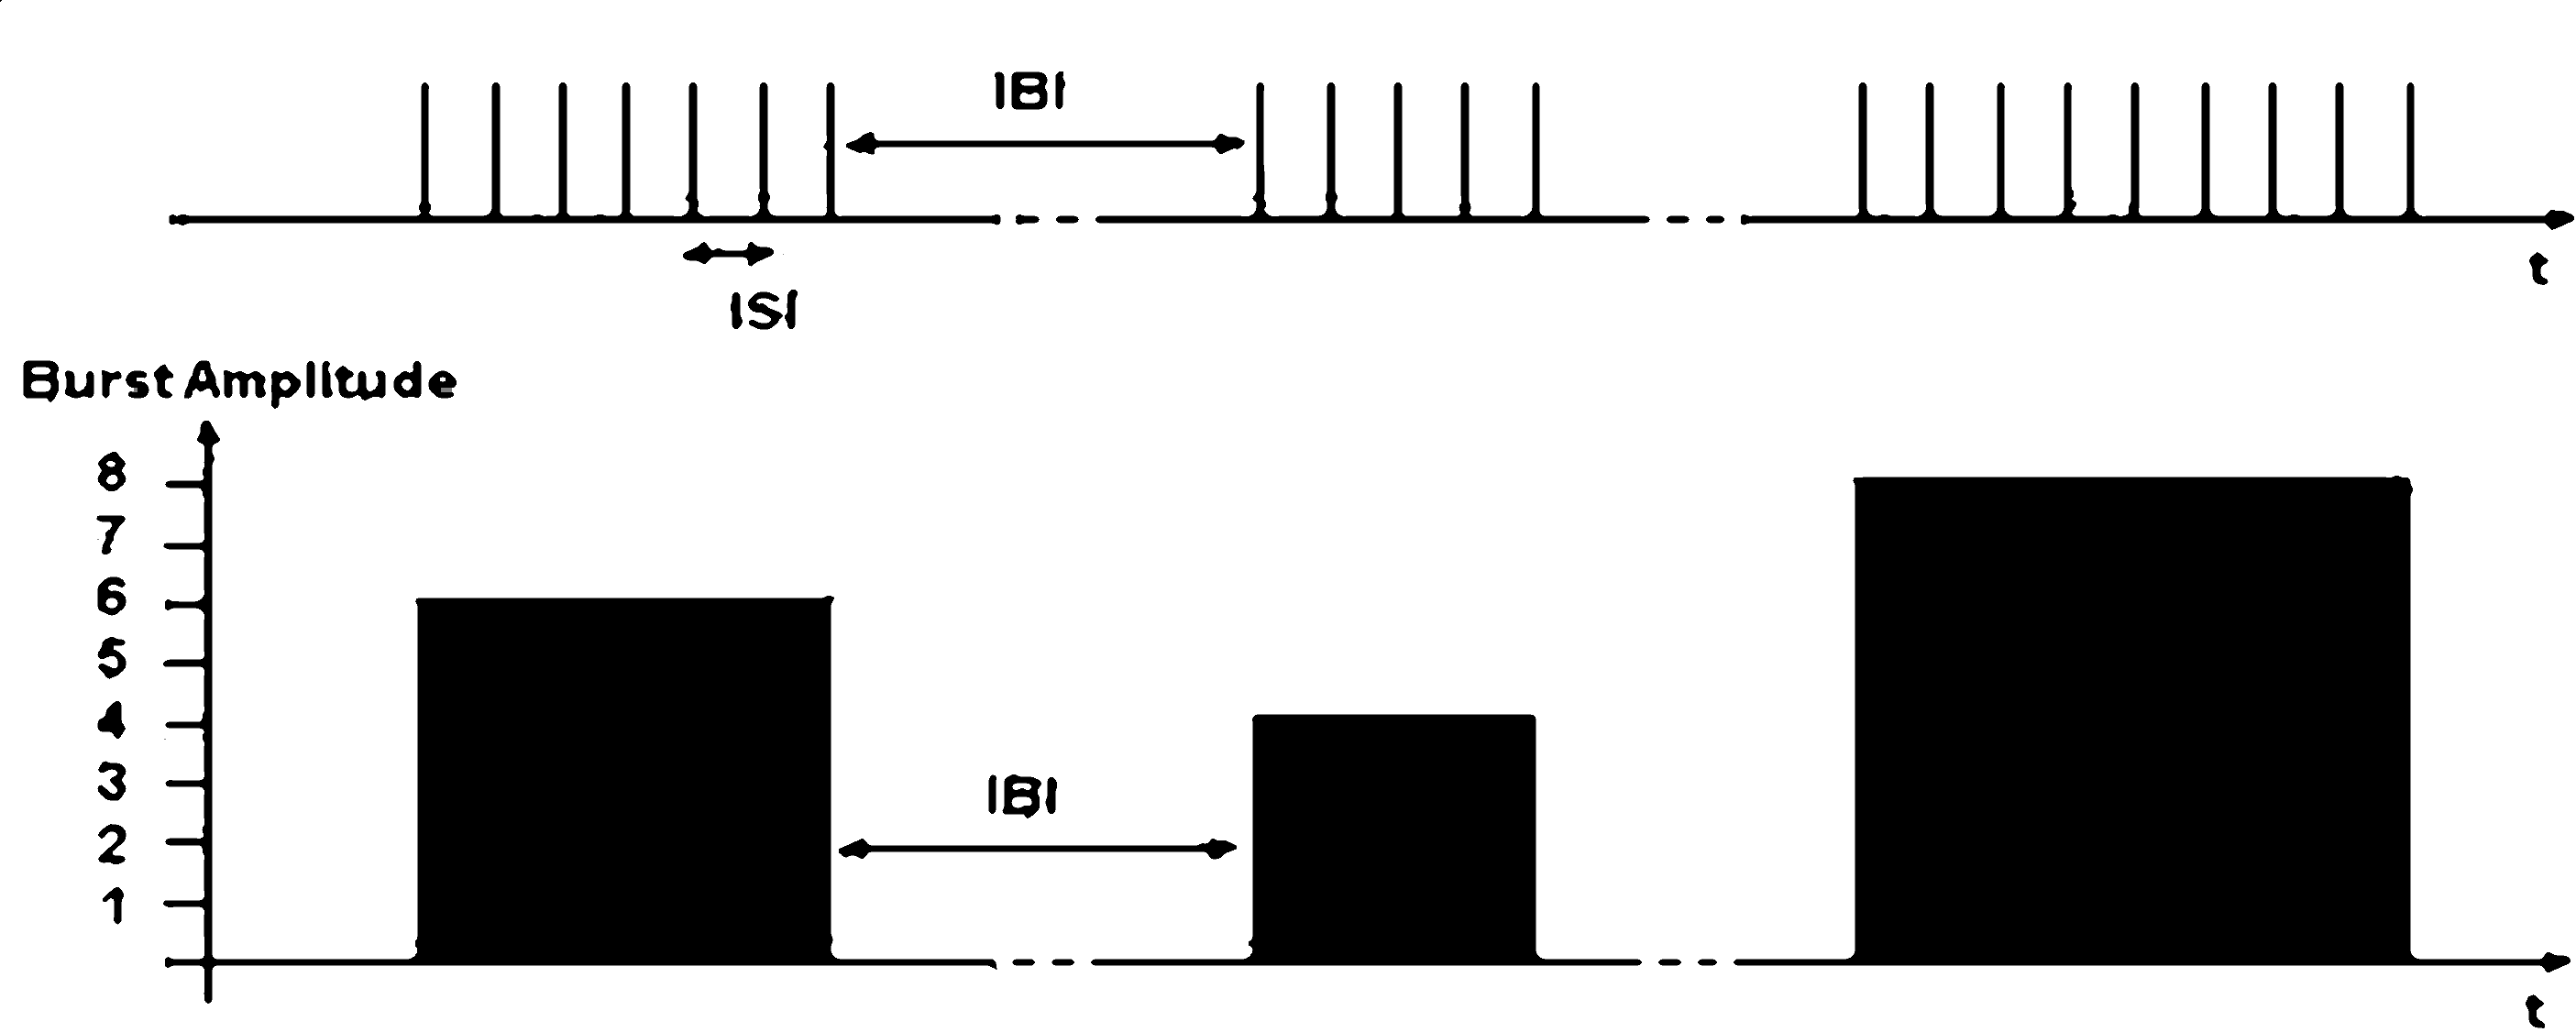
\includegraphics[scale=0.25]{5_2}
    \centering
\end{figure}
From a mathematical point of view, some properties can be extracted from a burst, such as:
\begin{itemize}
    \item \(t_b\): the starting time of the burst.
    \item \(T_b\): the burst duration.
    \item \(A_b\): the burst amplitude, related to the spike frequency within the burst.
\end{itemize}
A \textbf{single-channel burst train \(BT(t)\)}can be defined as follow:
\begin{align*}
    BT(t) = \sum_{b=1}^{NB}A_b*\prod\biggl(\frac{t-t_b-\frac{T_b}{2}}{T_b}\biggr)
\end{align*}
with \(NB\) being the number of detected bursts.
The amplitude \(A_b\) of the burst is computed as:
\begin{align*}
    A_b=\frac{1}{T_b}\int_{t_b}^{t_b+T_b}\sum_{s=1}^{N}\delta{(t-t_s)}\,dt=\frac{N_{T_b}}{T_b}
\end{align*}
where \(N_{T_b}\) is the number of spikes within the considered burst.\\
Notice that if the burst is defined in this way, it can be represented as a sequence of rectangles:
\begin{figure}[H]
    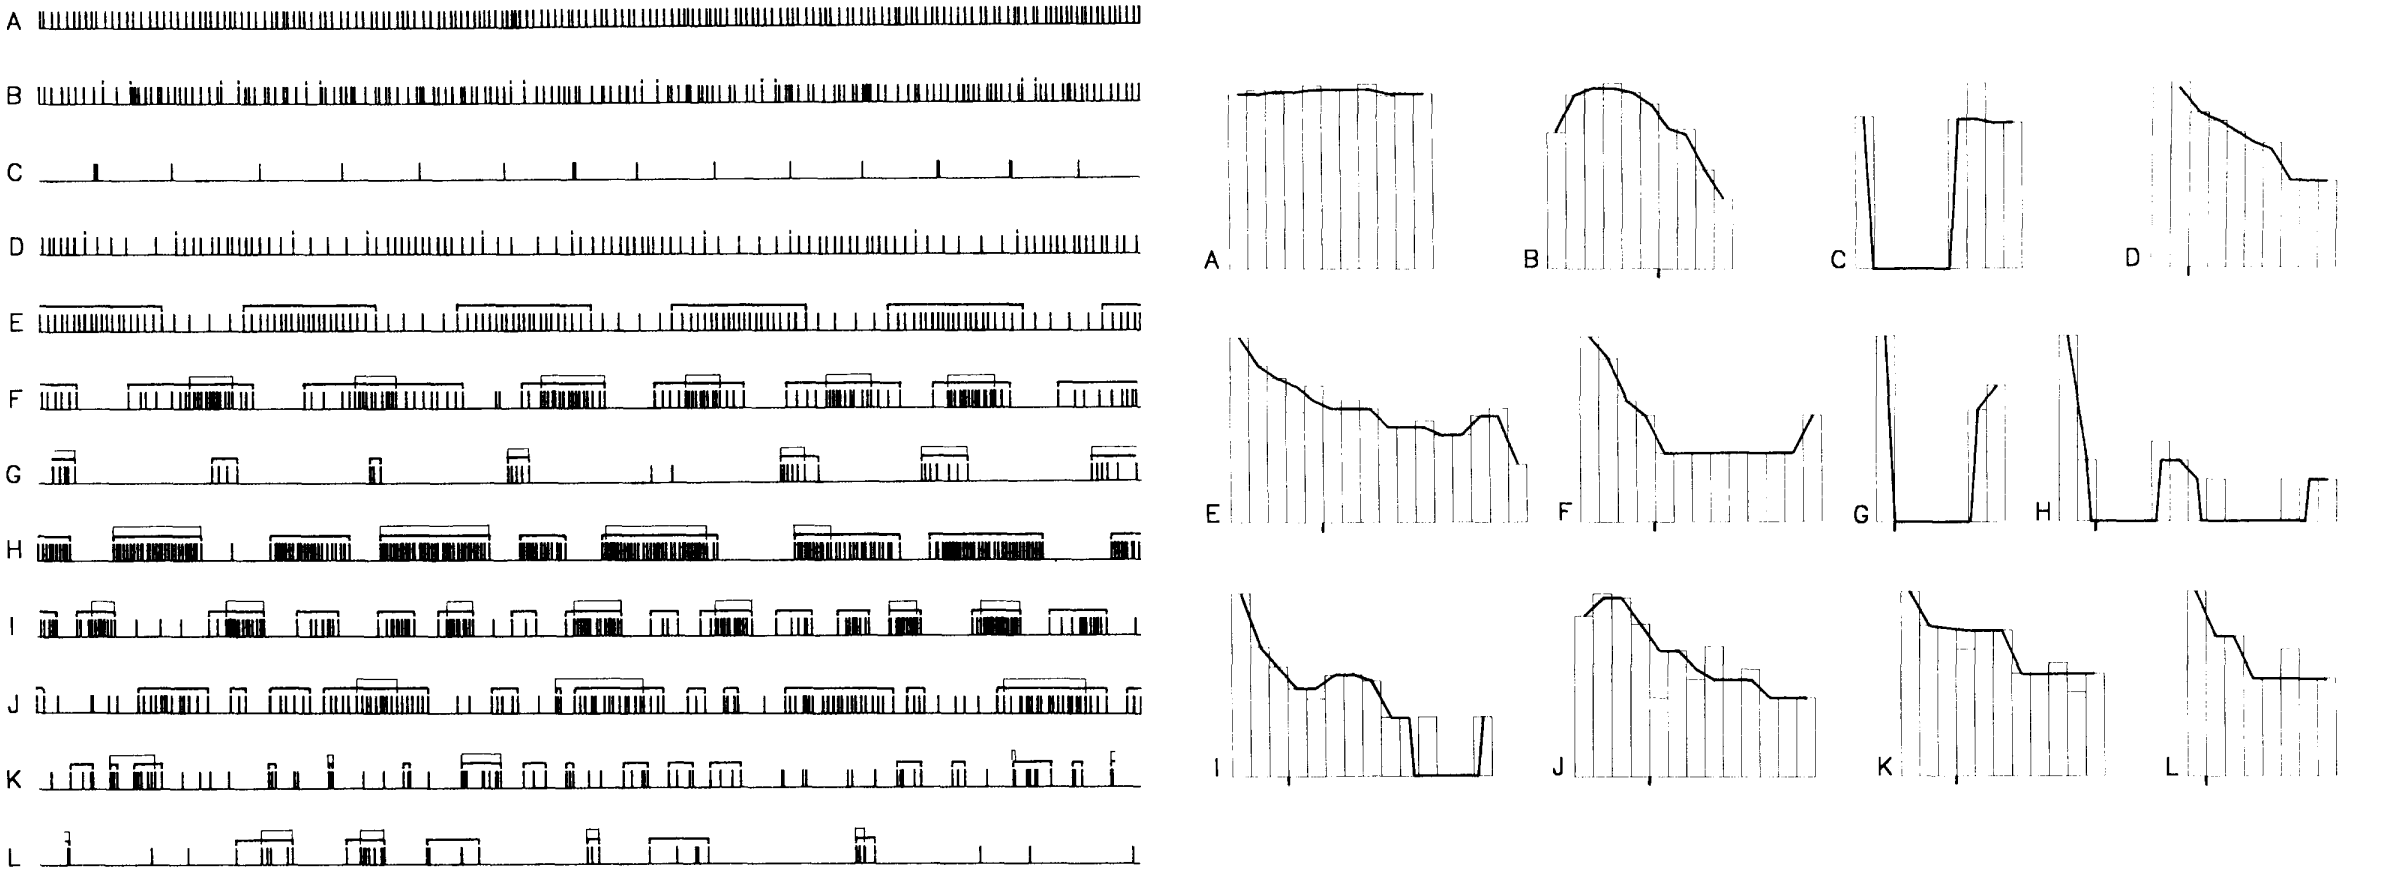
\includegraphics[scale=0.2]{5_3}
    \centering
\end{figure}
For the multi-channel case (\(M\) channels are considered), the burst train
expression can be easily modified:
\begin{align*}
    BT_{j}(t) = \sum_{b=1}^{NB_{j}}A_b*\prod\biggl(\frac{t-t_b-\frac{T_b}{2}}{T_b}\biggr)
    \quad\quad\text{with}\,j=1,...,M
\end{align*}
\subsubsection{Burst Event}
Another meaningful way to represent bursts is the \textbf{burst event train \(BE(t)\)}, which can be defined as a point process in which each event corresponds to the starting time of a burst. It is similar to a spike train, even if the meaning is different. 
A single-channel burst event train is defined as
\begin{align*}
    BE(t)=\sum_{b=1}^{NB}\delta(t-t_b)
\end{align*}
Hence, to find a burst event, the first spike of each burst (\(t_b\)) needs to be found.\\
In the case the channels are multiple \(M\), the definition can simply be extended:
\begin{align*}
    BE_{j}(t)=\sum_{b=1}^{NB_{j}}\delta(t-t_b)
    \quad\quad\text{with}\,j=1,...,M
\end{align*}


\subsection{Burst Detection Algorithms}
There are several algorithms to identify bursts.
\subsubsection{String Method} 
This algorithm is based on some hypotheses:
\begin{enumerate}
    \item \textbf{A burst is characterized by a certain number of spikes} \(\rightarrow\) the minimum number of spikes belonging to a burst needs to be defined.
    \item \textbf{Spikes in a burst are very close} \(\rightarrow\) a maximum ISI value has to be set, to consider a spike as a part of a or not.
    \item \textbf{Bursts are far away at least hundreds of ms} \(\rightarrow\) a minIBI has to be set, to consider 2 bursts as separated or not.
\end{enumerate}
Typically, the following values are selected:
\begin{itemize}
    \item \(ISI_{max}=100\,ms\)
    \item Minimum number of intra-burst spikes \(=5\)
    \item For simplicity, \(IBI_{min}=ISI_{max}\)
\end{itemize}
Because this method has a minimal computation time, it allows the implementation of burst analysis in real-time, including statistical changes in burst variables, histograms of burst types, and patterns in combinations of burst variables.
\subsubsection{Wagenaar (WA)} 
The method developed in 2005 by D. A. Wagenaar tries to solve a problem caused by the fact that usually bursts are characterized by two main trends:
at the beginning (\textbf{burst core}) the spiking frequency is particularly high, while
it tends to become increasingly low as time passes (\textbf{burst tail}). In order to
better detect the bursts accounting for the differences of the two portions just described, a system considering two distinct ISI thresholds is employed. \\
The steps carried out by the algorithm are:
\begin{enumerate}
    \item Set the mean firing rate \(f\). If the signal is multi-channel, set \(f_j\) for the \(j\)-th channel.
    \item Define a maximum core ISI. Often the following values are used: \(th_{core}=1/4f\) or \(th_{core}=100\,ms\). The factor 4 ensures that only spikes that succeed each other faster than 4 times the average firing rate can be considered as part of the channel burst.
    \item Look for sequences having at least a minimum number of intra-burst spikes.
    \item Change the maximum ISI threshold to higher values, such as \(th_{tail}=1/3f\) or \(th_{tail}=200\,ms\).
    \item Keep looking for spikes before and after the burst core satisfying the
          new threshold condition.
\end{enumerate}
\subsubsection{Cocatre-Zilgien and Delcomyn (CZ)} 
It represents the first method based on the analysis of the ISI histogram, as it is highly informative about the spiking pattern of a specific recording channel, as shown in the picture below. In particular, it analyzes the histogram to detect the \textbf{critical interval value} in the distribution that represents the break between short intervals within a burst and longer intervals between bursts. When such a value is found, it is used as the 'threshold' to determine those intervals in the spike train that lie within a burst and those that lie between bursts and, thereby, to identify the beginning and end of each burst in the train. So, bursting activity tends to result in valleys.
\begin{figure}[H]
    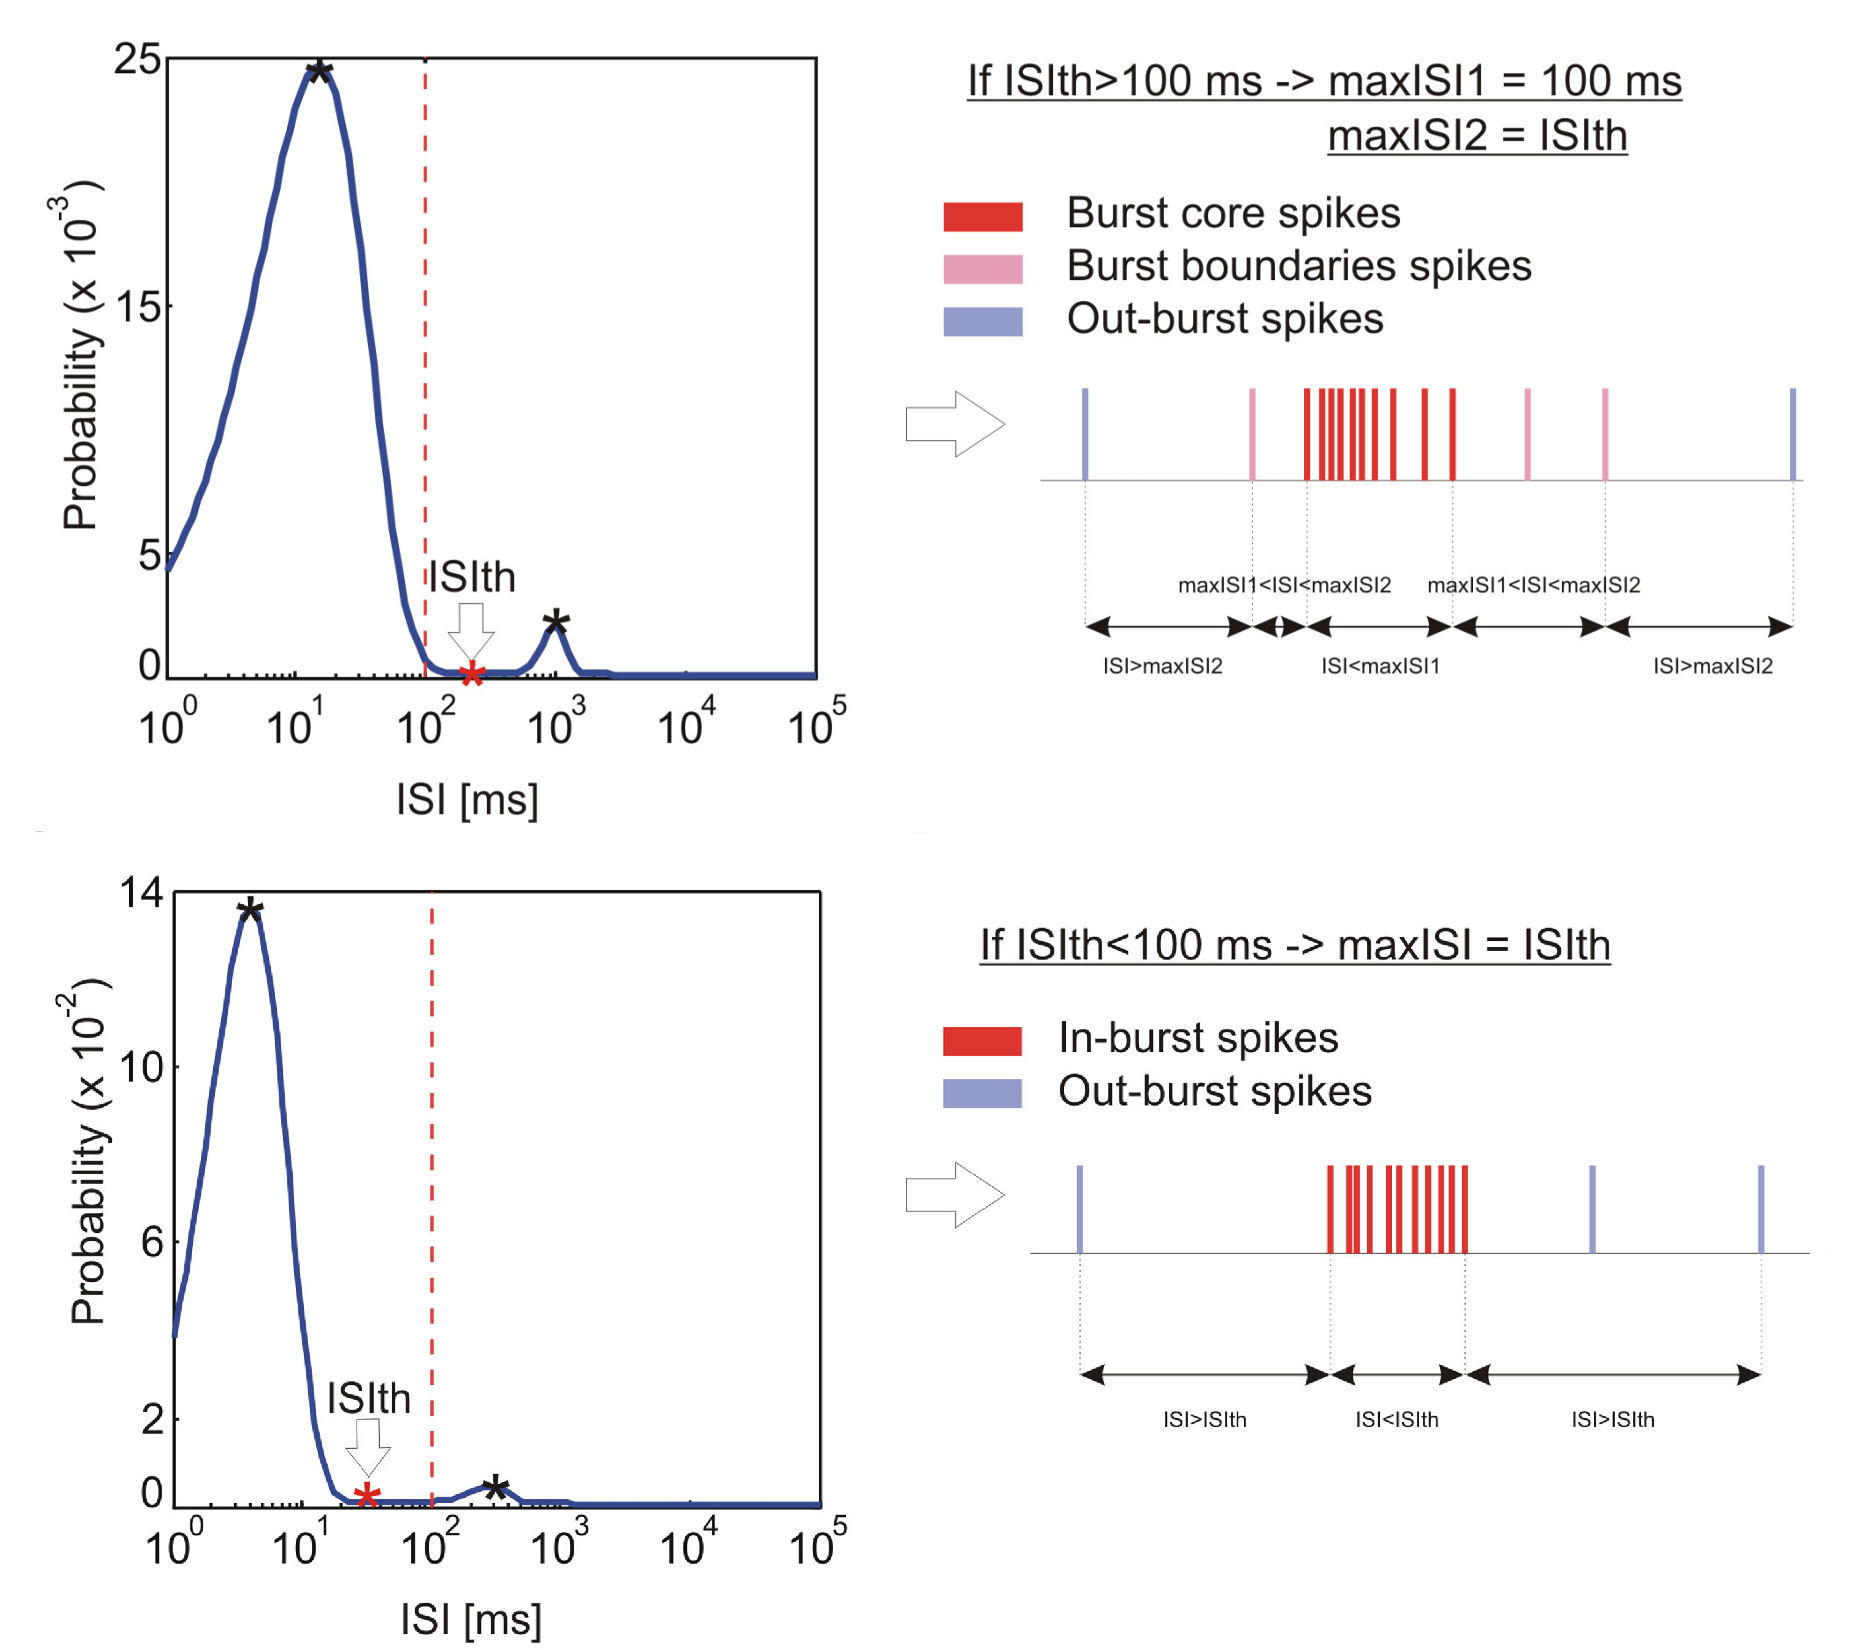
\includegraphics[scale=0.32]{5_5}
    \centering
\end{figure}

\subsubsection{Selinger (SE)} 
This method exploits the ISI histogram (in a logarithmic scale) to derive the optimal ISI threshold, then it works as a standard single threshold algorithm. This technique tries to improve the identification of the spikes in the tail portion of a burst.
\begin{figure}[H]
    \includegraphics[scale=0.5]{5_6}
    \centering
\end{figure}

\subsubsection{Modified Selinger (SE-MOD)} 
It is a modified version of the Selinger method, consisting in a mix of the already presented techniques. It allows a better identification of the spikes at the boundaries of a burst event.
\begin{figure}[H]
    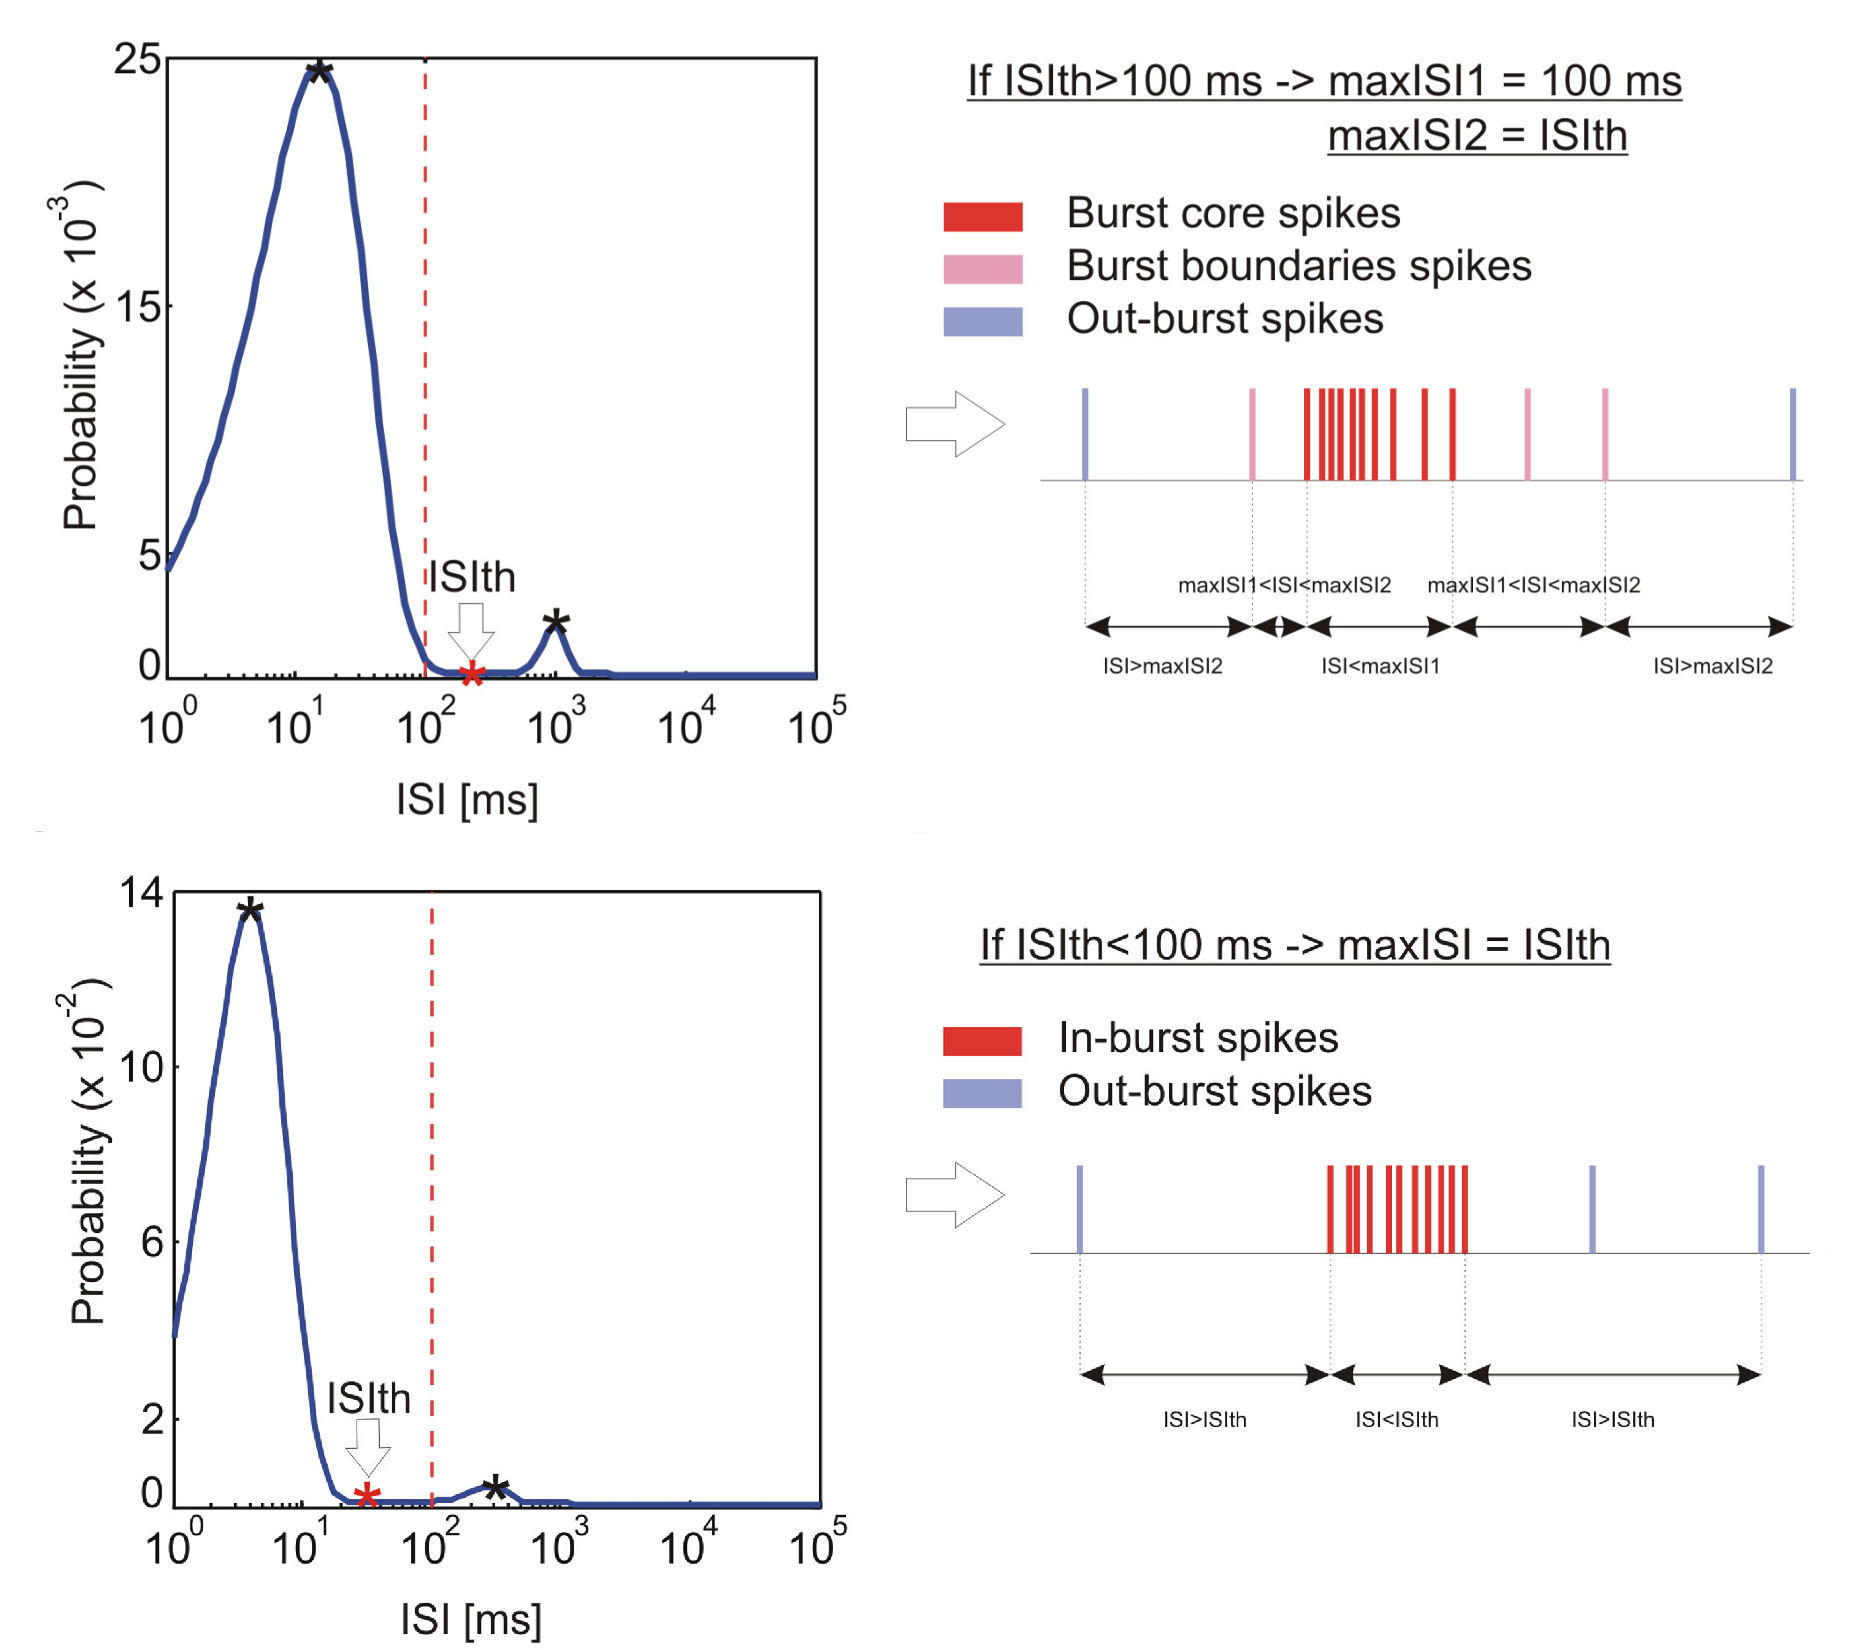
\includegraphics[scale=0.25]{5_7}
    \centering
\end{figure}
The asterisks in black represent the peaks and the one in red is the best point to separate the spikes (ISIth). If there is a burst, the approximation with the rectangular function is good from a mathematical point of view but, in reality, there are also some spikes with a lower frequency that yet belong to the burst.\\
With the string method, it's not always possible to detect all the spikes that belong to the burst. This because just a single threshold is used. Hence, it's better to define two of them: the \textbf{core} and the \textbf{tail thresholds}. The first is shorter, around \(100\,ms\), while the second is longer, between \(100\,ms\) and the ISIth. Obviously, this latter condition exists only if the ISIth is higher than \(100\,ms\). 
\begin{figure}[H]
    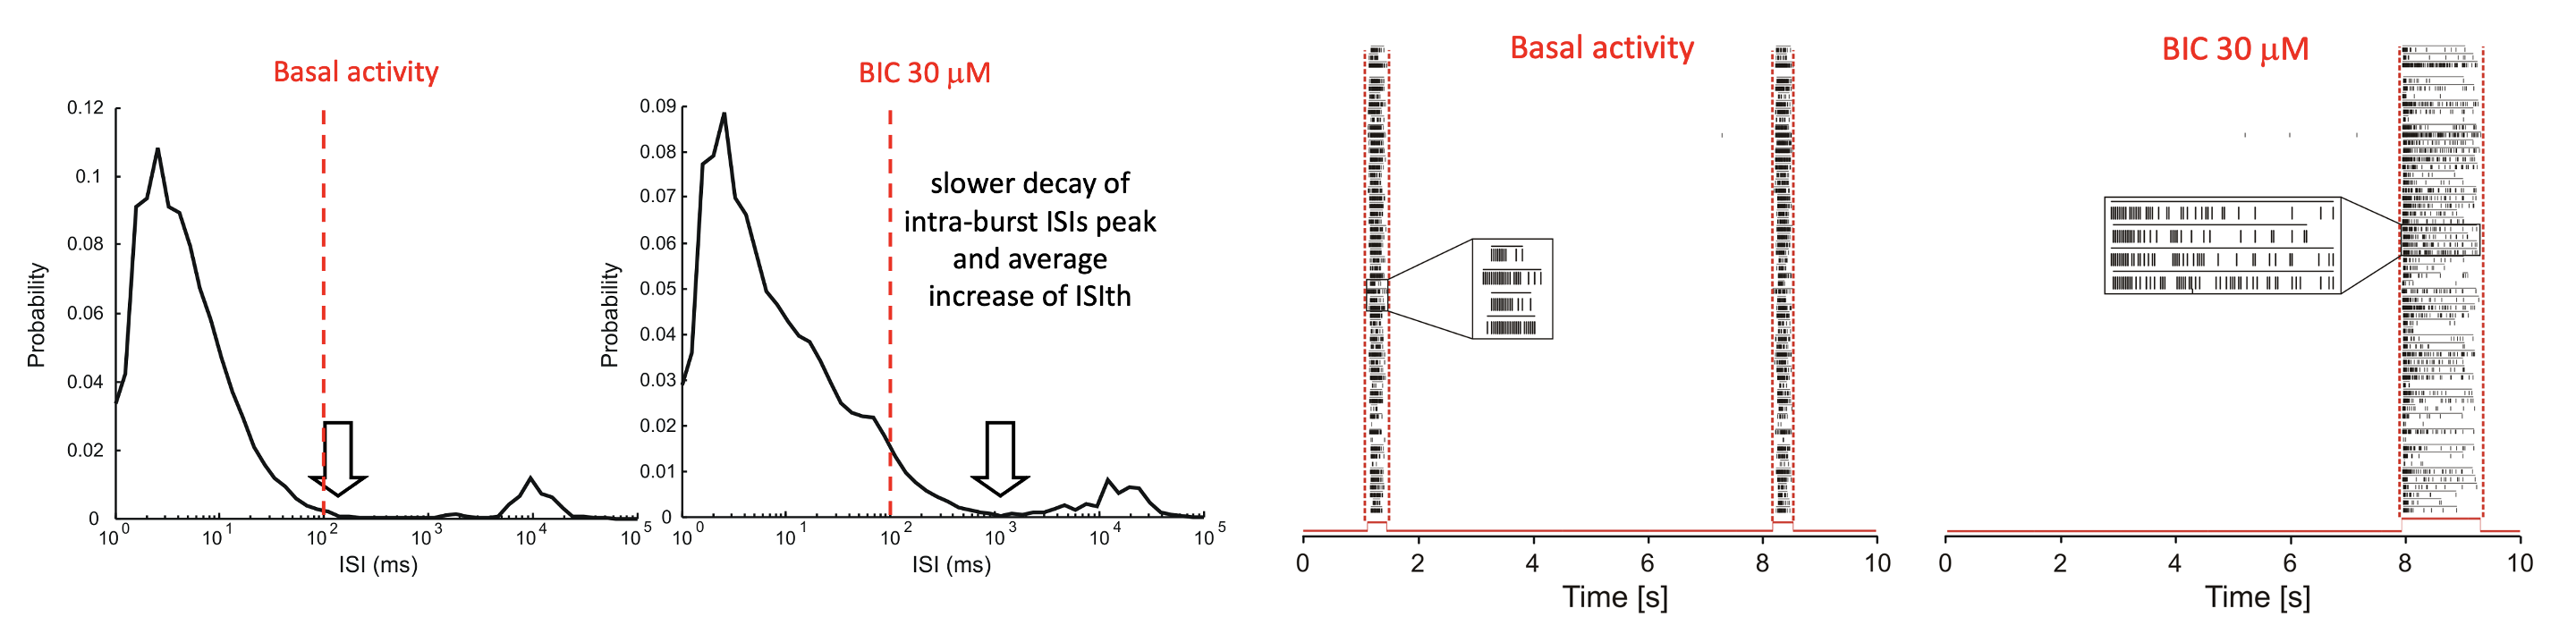
\includegraphics[scale=0.35]{5_8}
    \centering
\end{figure}
These images show recordings from in vitro culture, in particular the spontaneous activity (basal) and the activity
of an antagonist. In this second case there is a very long bursting activity.\\
It can be observed that from the basal to the antagonist activity there is a shift of the threshold. Moreover, notice that there are 2 peaks in the ISIh, that represent the two activities that can be observed in the bursts, where there is an area where the spikes are one near the other and another area in which they are more distant. The logISI algorithm is able to detect both cases. 

\subsection{Comparison of Algorithms}
Generally, it can be stated that all the implemented burst detection techniques proposed so far presents pros and cons, thus there is not an algorithm clearly prevailing on the others: different techniques perform better in different situations, according to the type of data that are intended to be analyzed.
\begin{figure}[H]
    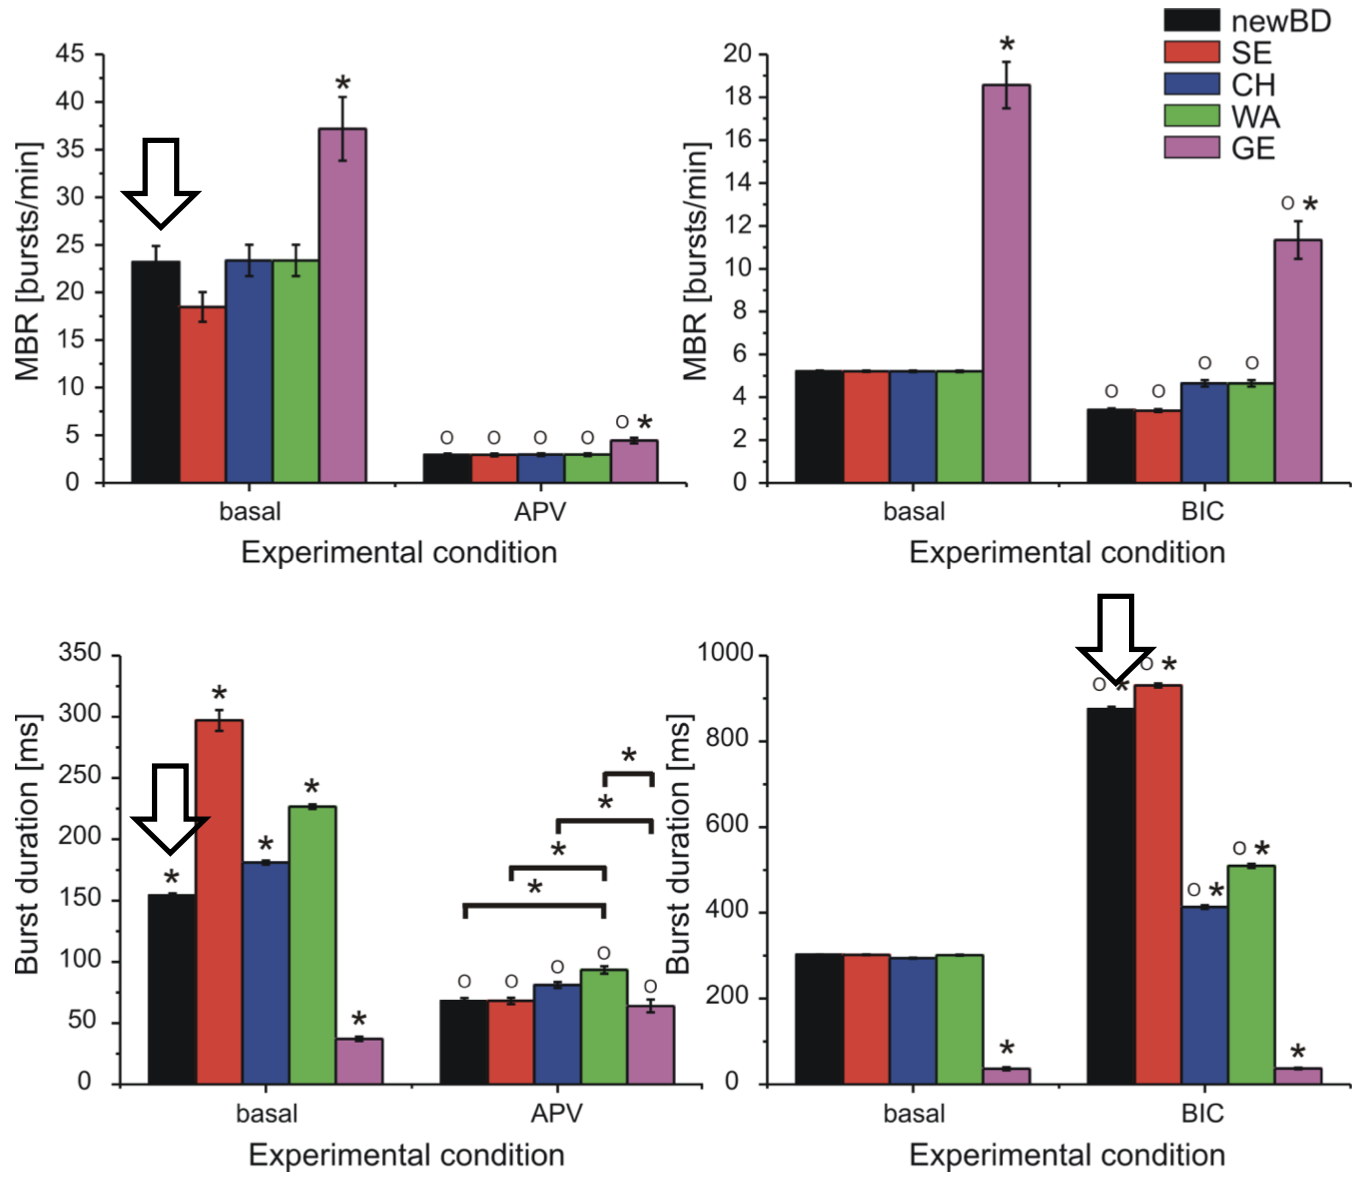
\includegraphics[scale=0.3]{5_9}
    \centering
\end{figure}
In the previous image, a quantitative comparison among the algorithms is realized:
\begin{itemize}
    \item the asterisk compares statistical differences in the same group.
    \item the empty circle compares the results of a specific method in different experimental conditions.
\end{itemize}
What can be deduced is that:
\begin{itemize}
    \item The logISI (newBD) algorithm is able to reveal the strong increase of burst duration caused by BIC stimulation, as the SE algorithm, whereas WA and CH fail.
    \item At the same time, in the basal condition of APV experiment, the logISI detects the 'correct' number of bursts (as WA and CH), whereas the SE algorithm fails.
    \item Finally, the GE algorithm provides clearly wrong burst detection when applied to in vitro recordings of neuronal cultures.
\end{itemize}